\section{ローズ・ピアノの簡易物理モデル}

本章ではローズ・ピアノ振動体を簡略化した物理モデルを検討する.簡易モデルに使用するシステムモデルを図\ref{fig:簡易モデル}に示す.

\begin{figure}
    \centering
    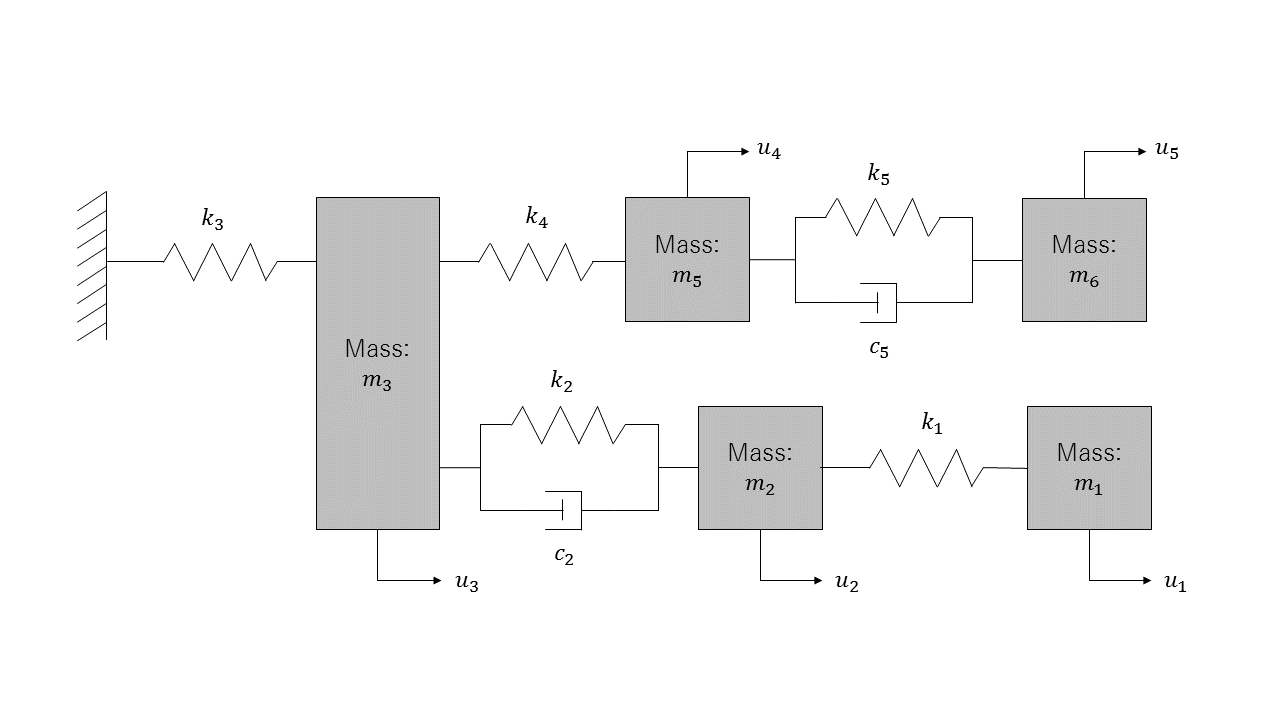
\includegraphics[width=15cm]{img/system-model.png}
    \caption{ローズ・ピアノの簡易物理モデル}
    \label{fig:簡易モデル}
\end{figure}


図はローズ・ピアノのシステムモデルである.$k$はバネ定数,$m$は質量,$u$は変位,$c$はダッシュポット,$l$は節の長さである.図中上部がTonebarになり,図中下部がTineに相当する.TonebarとTineをつないでいるPoleは$m_3$に相当する.

本章では,ローズ・ピアノのシステムモデルを連立常微分方程式として表し,TineとTonebarの連成振動を考慮した簡易物理モデルを提案する.



\subsection{連立常微分方程式}

主変数 $u$ に関する連立常微分方程式は,

\begin{equation}
    M \frac{d^2 u}{dt^2} + B_c^T R B_c \frac{du}{dt} + B_k^T D B_k = f    
\end{equation}

である.$M$は質量マトリクス,$D$はバネマトリクス,$R$は減衰マトリクス,$B_c$と$B_k$は剛性マトリクス,$f$は荷重マトリクスである.連立常微分方程式を粘弾性の運動方程式で一般化すると

\begin{eqnarray}
    m\ddot{u} + c\dot{u} + ku = f
\end{eqnarray}

である.$u$は質点の変位,$m$は質点の質量,$c$は減衰,$k$はバネ定数である.微分形式を省略するため,特に明記がない限り2階の時間微分は$\ddot{u}$,1階の時間微分は$\dot{u}$で表す.

図\ref{fig:簡易モデル}より,運動方程式からなる連立方程式は

\begin{eqnarray}
    \begin{matrix}
        m_1 \ddot{u_1} &+&  & & k_1 (u_1 - u_2) &=& 0 \\ 
        m_2 \ddot{u_2} &+& c_2(\dot{u_2} - \dot{u_3}) &+& k_2 (u_2 - u_3) - k_1 (u_2 - u_1) &=& 0 \\ 
        m_3 \ddot{u_3} &+& c_2(\dot{u_3} - \dot{u_2}) - c_3(\dot{u_3} - \dot{u_4}) &+& k_2 (u_3 - u_2) - k_3 (u_3 - u_4) &=& 0 \\ 
        m_4 \ddot{u_4} &+& c_3(\dot{u_4} - \dot{u_3}) &+& k_3 (u_4 - u_3) - k_5 (u_4 - u_5) - k_4 u_4 &=& 0 \\ 
        m_5 \ddot{u_5} &+& c_6(\dot{u_5} - \dot{u_6}) &+& k_6 (u_5 - u_6) - k_5 (u_5 - u_4) &=& 0 \\
        m_6 \ddot{u_6} &+& c_6(\dot{u_6} - \dot{u_5}) &+& k_6 (u_6 - u_5) &=& 0 \\
        m_7 \ddot{u_7} &+& c_7(\dot{u_7} - \dot{u_3}) & & &=& 0
    \end{matrix}        
\end{eqnarray}

である.連立方程式は変位に着目したとき,対象の変数と接続する変位との差を取ることで求まる.例えば,$u_2$の$c_2$及び$k_2$に着目するならば,$u_2$と接続している変位$u_3$について式を立てると,$c_2(\dot{u_2} - \dot{u_3})$と$k_2(u_2 - u_3)$が得られる.同じように$u_2$と接続している$u_1$に着目すると,$u_1$を接続しているのは$k_1$だけなので減衰項は$0$として$k_2(u_2 - u_1)$だけが得られる.それぞれの項を足し合わせると$u_2$に関する運動方程式を立てられる.これをすべての変位で繰り返すと連立方程式となる.

運動方程式より状態方程式は,

\begin{eqnarray}
    u = 
    \left[\begin{matrix}
        u_1 \\
        u_2 \\
        u_3 \\
        u_4 \\
        u_5 \\
        u_6 \\
        u_7 \\
        u_8
    \end{matrix}\right]
\end{eqnarray}

\begin{eqnarray}
    f = 
    \left[\begin{matrix}
        f_1 \\
        f_2 \\
        f_3 \\
        f_4 \\
        f_5 \\
        f_6 \\
        f_7 \\
        f_8
    \end{matrix}\right]
\end{eqnarray}

\begin{eqnarray}
    M = 
    \left(\begin{matrix}
        m_1 & 0   & 0   & 0   & 0   & 0   & 0   & 0   \\
        0   & m_2 & 0   & 0   & 0   & 0   & 0   & 0   \\
        0   & 0   & m_3 & 0   & 0   & 0   & 0   & 0   \\
        0   & 0   & 0   & m_4 & 0   & 0   & 0   & 0   \\
        0   & 0   & 0   & 0   & m_5 & 0   & 0   & 0   \\
        0   & 0   & 0   & 0   & 0   & m_6 & 0   & 0   \\
        0   & 0   & 0   & 0   & 0   & 0   & m_7 & 0   \\
        0   & 0   & 0   & 0   & 0   & 0   & 0   & m_8  
    \end{matrix}\right)
\end{eqnarray}

\begin{eqnarray}
    D =
    \left(\begin{matrix}
        k_1 & 0   & 0   & 0   & 0   & 0   & 0   & 0   \\
        0   & k_2 & 0   & 0   & 0   & 0   & 0   & 0   \\
        0   & 0   & k_3 & 0   & 0   & 0   & 0   & 0   \\
        0   & 0   & 0   & k_4 & 0   & 0   & 0   & 0   \\
        0   & 0   & 0   & 0   & k_5 & 0   & 0   & 0   \\
        0   & 0   & 0   & 0   & 0   & k_6 & 0   & 0   \\
        0   & 0   & 0   & 0   & 0   & 0   & 0   & 0   \\
        0   & 0   & 0   & 0   & 0   & 0   & 0   & k_8
    \end{matrix}\right)
\end{eqnarray}

\begin{eqnarray}
    R = 
    \left(\begin{matrix}
        0   & 0   & 0   & 0   & 0   & 0   & 0   & 0   \\
        0   & c_2 & 0   & 0   & 0   & 0   & 0   & 0   \\
        0   & 0   & c_3 & 0   & 0   & 0   & 0   & 0   \\
        0   & 0   & 0   & 0   & 0   & 0   & 0   & 0   \\
        0   & 0   & 0   & 0   & 0   & 0   & 0   & 0   \\
        0   & 0   & 0   & 0   & 0   & c_6 & 0   & 0   \\
        0   & 0   & 0   & 0   & 0   & 0   & 0   & 0   \\
        0   & 0   & 0   & 0   & 0   & 0   & 0   & c_8
    \end{matrix}\right)
\end{eqnarray}

である.ただし,$u_8, f_8, m_8, k_8, c_8$は境界条件であるため$0$である.

剛性マトリクスは連立方程式にかかる剛性マトリクスから行列を作成し,重ね合わせの原理によって足し合わせることで求められる.単に$k$もしくは$c$に対して何倍なのか求めればいいだけであるため,連立方程式より

\begin{eqnarray}
    B_k = 
    \left(\begin{matrix}
        1   & -1  & 0   & 0   & 0  & 0  & 0  & 0  \\
        -1  & 2   & -1  & 0   & 0  & 0  & 0  & 0  \\
        0   & -1  & 2   & -1  & 0  & 0  & 0  & 0  \\
        0   & 0   & -1  & 3   & -1 & 0  & 0  & 0  \\
        0   & 0   & 0   & -1  & 2  & -1 & 0  & 0  \\
        0   & 0   & 0   & 0   & -1 & 1  & 0  & 0  \\
        0   & 0   & 0   & 0   & 0  & 0  & 0  & 0  \\
        0   & 0   & 0   & 0   & 0  & 0  & 0  & 0  
    \end{matrix}\right)
\end{eqnarray}

\begin{eqnarray}
    B_c = 
    \left(\begin{matrix}
        0   & 0   & 0   & 0   & 0  & 0  & 0  & 0  \\
        0   & 1   & -1  & 0   & 0  & 0  & 0  & 0  \\
        0   & -1  & 2   & -1  & 0  & 0  & 0  & 0  \\
        0   & 0   & -1  & 1   & 0  & 0  & 0  & 0  \\
        0   & 0   & 0   & 0   & 1  & -1 & 0  & 0  \\
        0   & 0   & 0   & 0   & -1 & 1  & 0  & 0  \\
        0   & 0   & -1  & 0   & 0  & 0  & 1  & 0  \\
        0   & 0   & 0   & 0   & 0  & 0  & 0  & 0  
    \end{matrix}\right)
\end{eqnarray}

が得られる.よって,

\begin{eqnarray}
    M\ddot{u} =
    \left[\begin{matrix}
        m_1 \ddot{u_1} \\
        m_2 \ddot{u_2} \\
        m_3 \ddot{u_3} \\
        m_4 \ddot{u_4} \\
        m_5 \ddot{u_5} \\
        m_6 \ddot{u_6} \\
        m_7 \ddot{u_7} \\
        m_8 \ddot{u_8} \\
    \end{matrix}\right]
\end{eqnarray}

\begin{eqnarray}
    B_k^T R B_k \dot{u} =
    \left[\begin{matrix}
        0 \\
        c_2 (\dot{u_2} - \dot{u_3}) + c_3 (\dot{u_3} - \dot{u_4}) \\
        c_3 (\dot{u_3} - \dot{u_4}) \\
        0 \\
        0 \\
        0 \\
        c_6 (\dot{u_6} - \dot{u_5}) \\
        c_7 (\dot{u_7} - \dot{u_3}) \\
        0
    \end{matrix}\right]
\end{eqnarray}

\begin{eqnarray}
    B_k^T D B_k u =
    \left[\begin{matrix}
        k_1 (u_1 - u_2) \\
        k_2 (u_2 - u_3) - k_1 (u_1 - u_2) \\
        k_3 (u_3 - u_4) - k_2 (u_2 - u_1) - k_1 (u_1 - u_2) \\
        k_4 u_4 - k_3 (u_3 - u_2) - k_2 (u_2 - u_1) - k_1 (u_1 - u_2) - k_5 (u_4 - u_5) - k_6 (u_5 - u_6) \\
        k_5 (u_5 - u_4) - k_6 (u_6 - u_5) \\
        k_6 (u_6 - u_5) \\
        0 \\
        0
    \end{matrix}\right]
\end{eqnarray}

である.
